\documentclass{article}
\usepackage{amsmath}
\usepackage{amsthm}
\usepackage{amsfonts}
\usepackage{amssymb}
\usepackage{bbold}
\usepackage{dsfont}
\usepackage{graphicx}
\usepackage{cleveref}
\usepackage{bm}
\usepackage{booktabs}
\usepackage{siunitx}
\usepackage{xcolor}
\usepackage[utf8]{inputenc}
\usepackage[english]{babel}
\newtheorem{definition}{Definition}
\newtheorem{example}{Example}
\newcommand{\exP}[1]{\mathrm{e}^{#1}}
\newcommand{\dif}{\mathrm{d}}
\renewcommand{\vec}[1]{\mathbf{#1}}
\newcommand{\pdagger}{{\phantom{\dagger}}}
\newcommand{\state}[1]{\vert #1\rangle}
\newcommand{\cstate}[1]{\langle #1\vert}
\newcommand{\tr}[1]{\mathrm{tr}\left\{#1\right\}}
\newcommand{\trs}[2]{\, \mathrm{tr}_{#1}\{#2\}}
\newcommand{\expc}[3]{\langle #1\vert #2 \vert #3\rangle}
\usepackage[doi=false,url=false,isbn=false,backend=bibtex,style=nature,natbib=true,sorting=none]{biblatex}
\bibliography{bib.bib}
\usepackage{geometry}
\geometry{
	a4paper,
	total={170mm,257mm},
	left=20mm,
	top=20mm,
}
\begin{document}
\title{Comparison between Ehrenfest and TTHEOM}
\author{Rudolf Smorka}
\maketitle
\section{$L=1\times 2$}
\Cref{fig:1} (a) shows the current and (b) the electronic spin polarization on site 1 for a system with size $L=1\times 2$. Other parameters are $\varepsilon_0 =- \SI{240}{\milli\electronvolt}, \omega_0 = \SI{2}{\milli\electronvolt}, t_0 = \SI{40}{\milli\electronvolt}, t_1 = 0.1t_0, \Gamma = \SI{10}{\milli\electronvolt}$ and $T=\SI{300}{\kelvin}$. The lead spin polarization is $P=0.5$. Both plots compare observables obtained with the Ehrenfest approach (red curve) with the TTHEOM approach (varying rank) and the exact result (for $t_1=0$, blue dashed line). A rank of $r=120$ is sufficient for convergence of the results up to $\sim \SI{200}{\femto\second}$. 
\begin{figure}[!h]
	\centering
	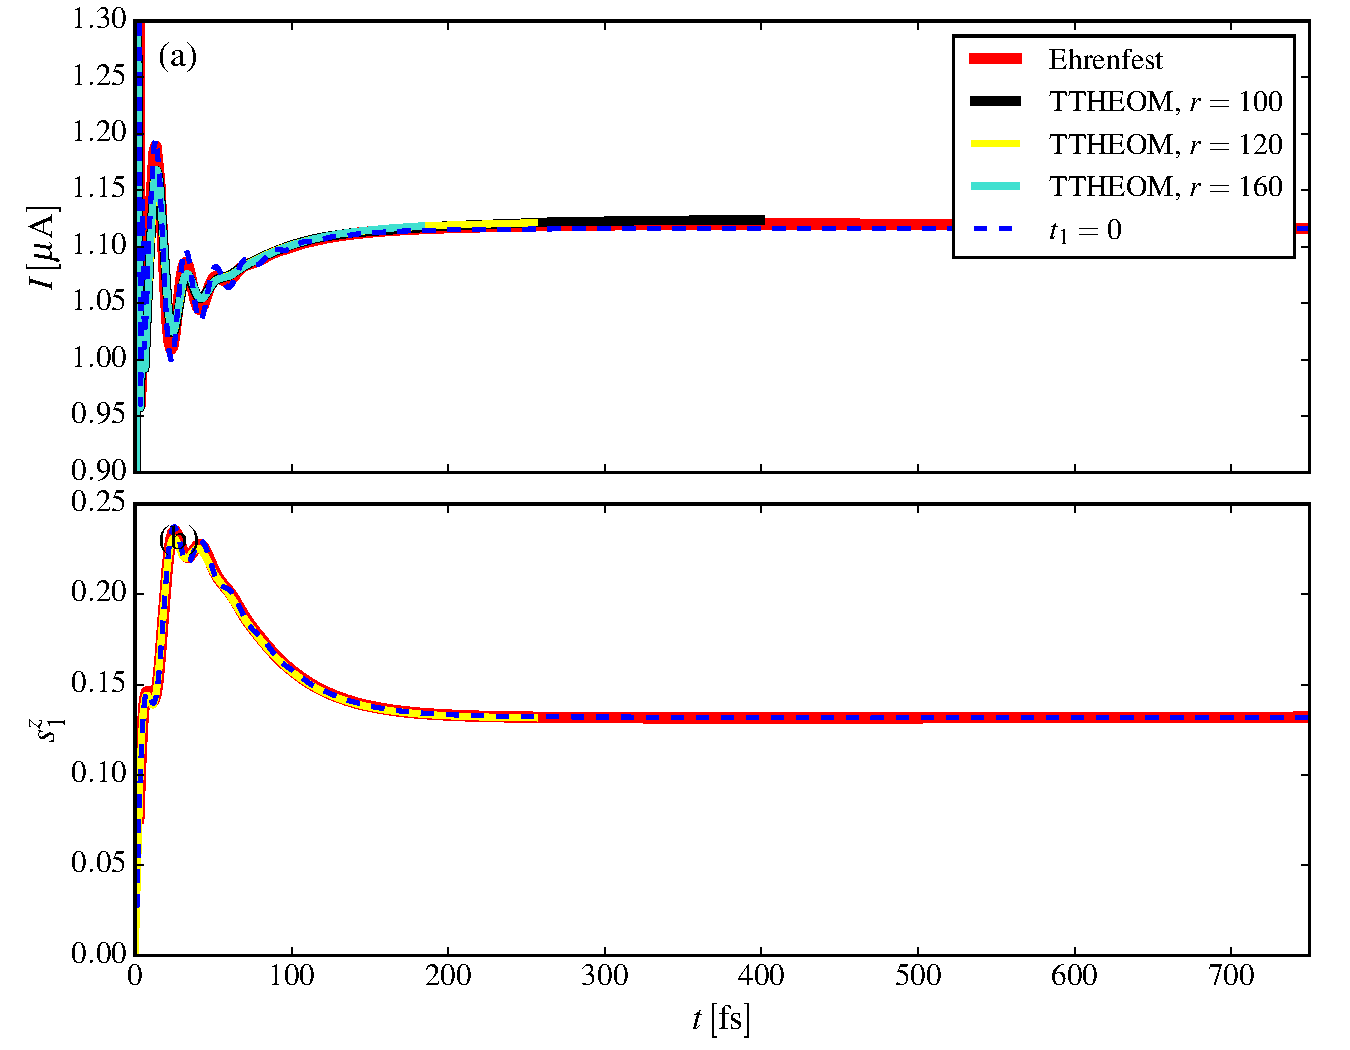
\includegraphics[width=0.9\textwidth]{figs/L2_comparison_TTHEOM_MFHEOM_v3_PVar.pdf}
	\caption{Ehrenfest: $n=1500$. TTHEOM: $n_\mathrm{vib}=30$. Initial state in both approaches: Empty molecule and vibration in zero temperature ground state.} \label{fig:1}
\end{figure}
\section{$L=1\times 3$}
\Cref{fig:2} shows the current and the electronic spin polarization for the same parameters as in the previous section, with spin orbit coupling parameter $\lambda_0=\SI{1}{\milli\electronvolt}$ and $\lambda_1 = \SI{0.1}{\milli\electronvolt}$ and for a system size $L=1\times 3$. \Cref{fig:3} shows the dynamics of the magnetoresistance $M_R$. In the Ehrenfest approach, the magnetoresistance for this system size is numerically zero. 
\begin{figure}[!h]
	\centering
	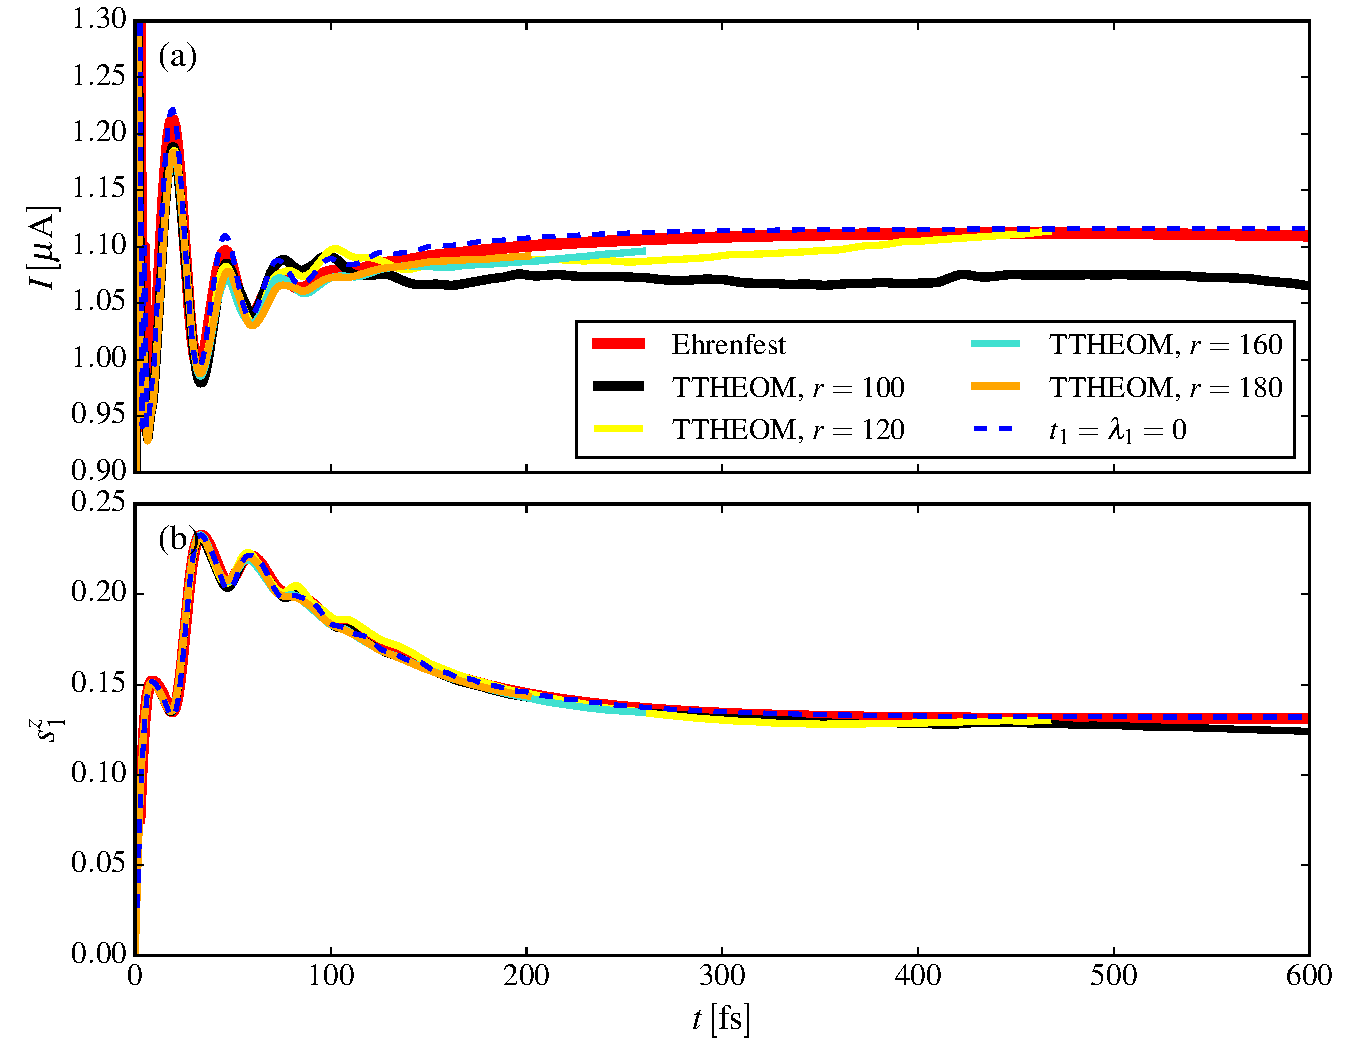
\includegraphics[width=0.9\textwidth]{figs/L3_comparison_TTHEOM_MFHEOM_v3_PVar.pdf}
	\caption{Ehrenfest: $n=1275$. TTHEOM: $n_\mathrm{vib}=30$. } \label{fig:2}
\end{figure}
\begin{figure}[!h]
	\centering
	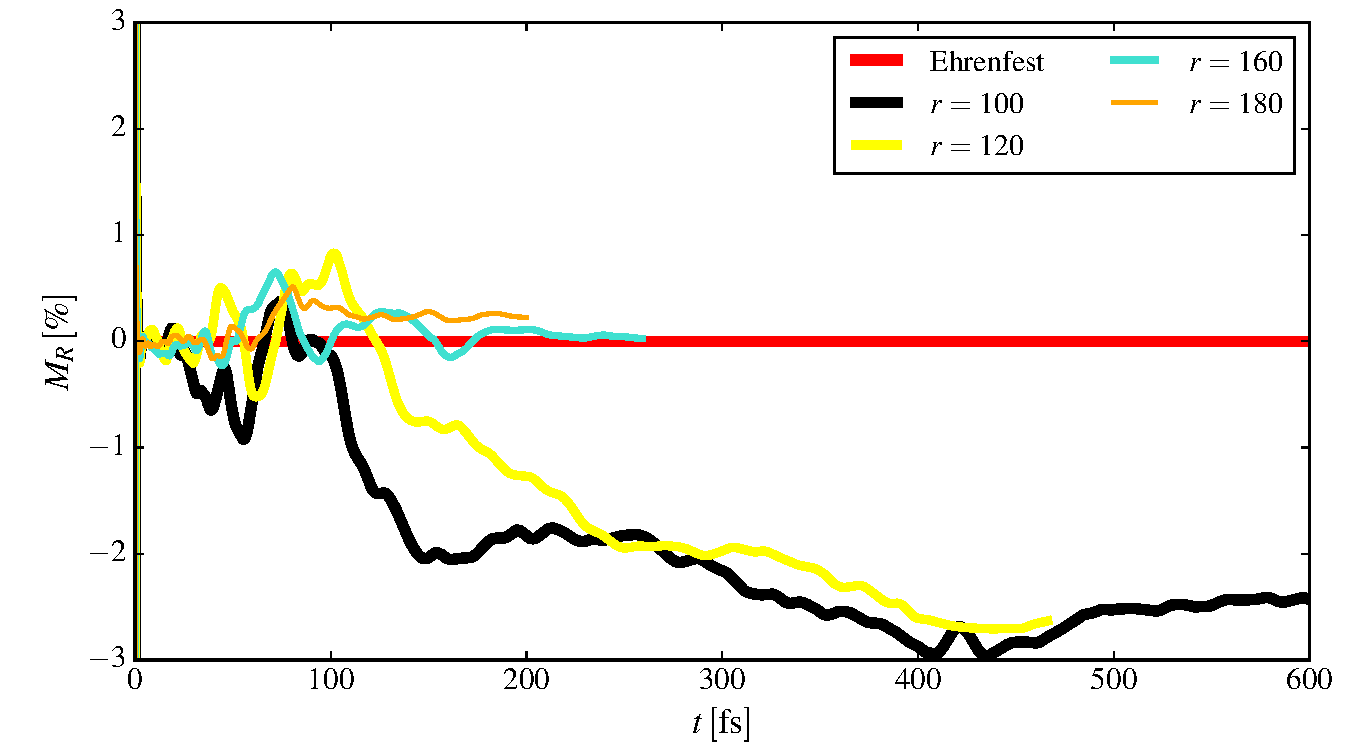
\includegraphics[width=0.9\textwidth]{figs/L3_comparison_MR_TTHEOM_PVar.pdf}
	\caption{Magnetoresistance. Ehrenfest: $n=1275$. TTHEOM: $n_\mathrm{vib}=30$.} \label{fig:3}
\end{figure}
\section{Norm of state}
The norm of the state at each time step $\langle \!\langle \mathds{1}\vert \rho(t)\rangle\!\rangle$ is shown in \cref{fig:4}. Solid lines depict the norm for $L=1\times 2$ and dashed ones for $L=1\times 3$. 
\begin{figure}[!h]
	\centering
	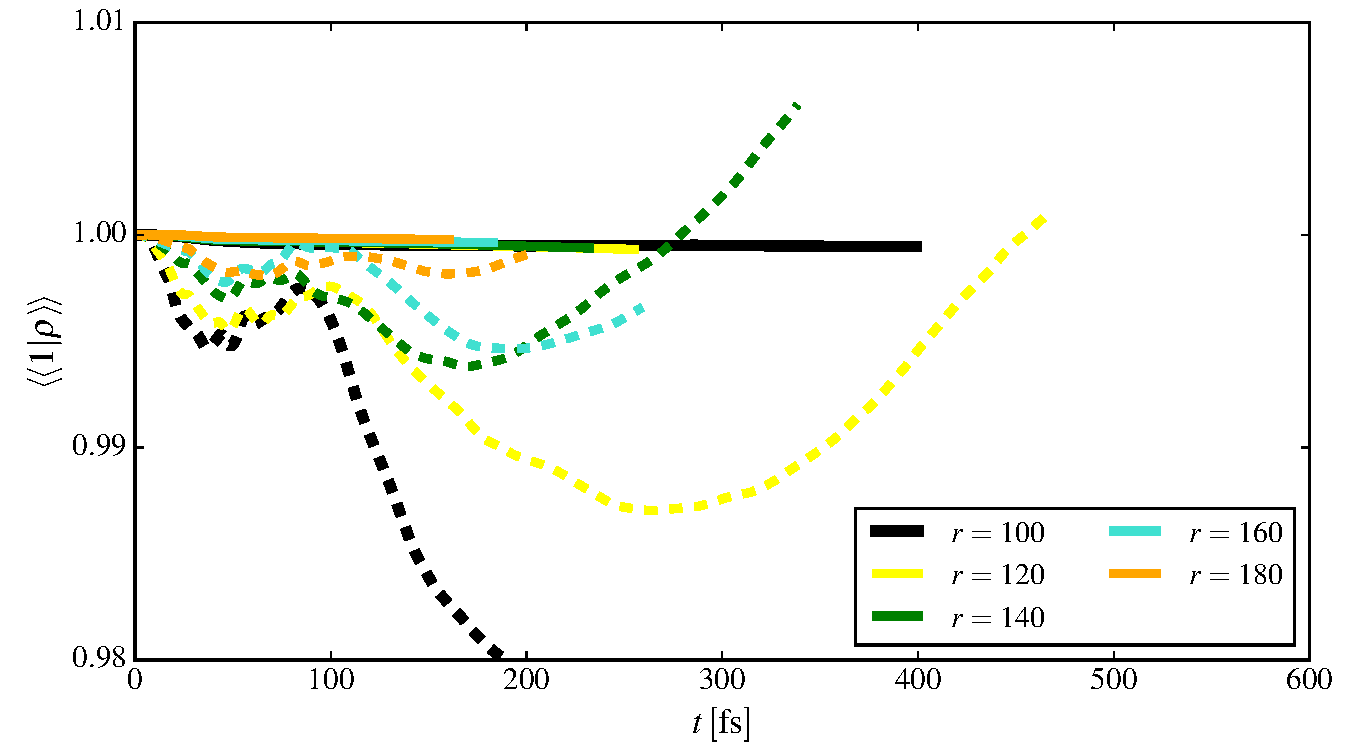
\includegraphics[width=0.9\textwidth]{figs/Norm_TTHEOM_rankVar_LVar.pdf}
	\caption{Norm of state for varying rank. Solid lines show $L=1\times 2$ and dashed ones $L=1\times 3$.}\label{fig:4}
\end{figure}
\printbibliography

\end{document}

